\section{Principle and ideas}
\label{sec:principle}

%\begin{itemize}
%    \item goal: expressive and safe (more expressive than and at least as safe
%        as eBPF)
%    \item Current problem of eBPF: the verifier
%    \item Idea: remove the verifier and use a safe language
%    \item the language should be Turing complete and at the same time low-level
%        enough to provide safety features.
%    \item We choose Rust as the implementation language.
%    \item The use of Rust automatically provides eexpresssiveness
%    \item We then show how a safety can be achieved for kernel extensions via
%        language-based safety from Rust.
%    \item how to ensure safety (high-level discussion, no implementation
%        details)
%        \begin{itemize}
%            \item builtin memory/control/type safety
%                \begin{itemize}
%                    \item generic and const-generic functions and slices to
%                        prevent OOB access
%                    \item Safe direct packet access for XDP programs
%                    \item Retired expressiveness kernel helpers (\jinghao{probably does not belong here})
%                \end{itemize}
%            \item RAII (e.g. lock, refcnt)
%            \item exception handling and stack unwinding
%                \begin{itemize}
%                    \item Needed because Rust itself has runtime checks (e.g.
%                        array OOB access)
%                    \item handle exceptional control flow
%                    \item clean up resources to achieve RAII under exceptional
%                        circumstances
%                \end{itemize}
%            \item runtime mechanism to support properties that are
%                (fundamentally) hard to check at compile time
%                \begin{itemize}
%                    \item program termination
%                    \item stack overflow protection
%                \end{itemize}
%        \end{itemize}
%\end{itemize}

The goal of \projname{} is to provide enhanced usuability for kernel extensions,
    while ensuring the safety properties of the extension programs.
In particular, we aim to make \projname{} more usable than eBPF and at least
    as safe as eBPF.
As discussed in \S~\ref{sec:motivation}, the current problem on usability of
    eBPF is the large semantic gap between the programer, who works on
    high-level langauges, and the verifier, which operates on compiled bytecode.
% Our insight is that both the needed expressiveness and safety can be obtained
%     from a safe programming language without the verifier.
Our insight is that by using a safe, high-level langauge that directly
    implements the required safety of the kernel, the semantic gap can be
    closed.
% Specifically, the language should have the following properties:
% \begin{itemize}
%     \item \textbf{Turing-complete}: This helps to satisfy the expressiveness
%         requirement.
%     \item \textbf{Safe}: The language should not be as permissive and
%         error-prone as unsafe languages like C.
%     \item \textbf{Low-level}: Being low-level helps the programs to better
%         model low-level kernel semantics and simplifies infrastructure needed
%         to support it.
% \end{itemize}
\projname{} uses Rust as the language for extension programs.
This is because Rust happens to provide the desired properties -- its
    langauge-based safety can be leveraged for safe kernel extensions without a
    verifier.
We now discuss how the safety properties from Rust can be applied to the
    context of kernel extensions to provide a safe programming interface.
% While the use of Rust automatically provides expressiveness (as it is
%     Turing-complete), it does not supply the safety out-of-box, and the use of
%     Rust, especially unsafe Rust, can still exhibit undesired behaviors.
% We require all extension programs to be implemented \textit{only} in safe Rust.
% On top of that, we discuss how the safety properties from Rust can be leveraged
%     and applied to the context of kernel extensions to provide a safe
%     programming interface.

\begin{figure}
    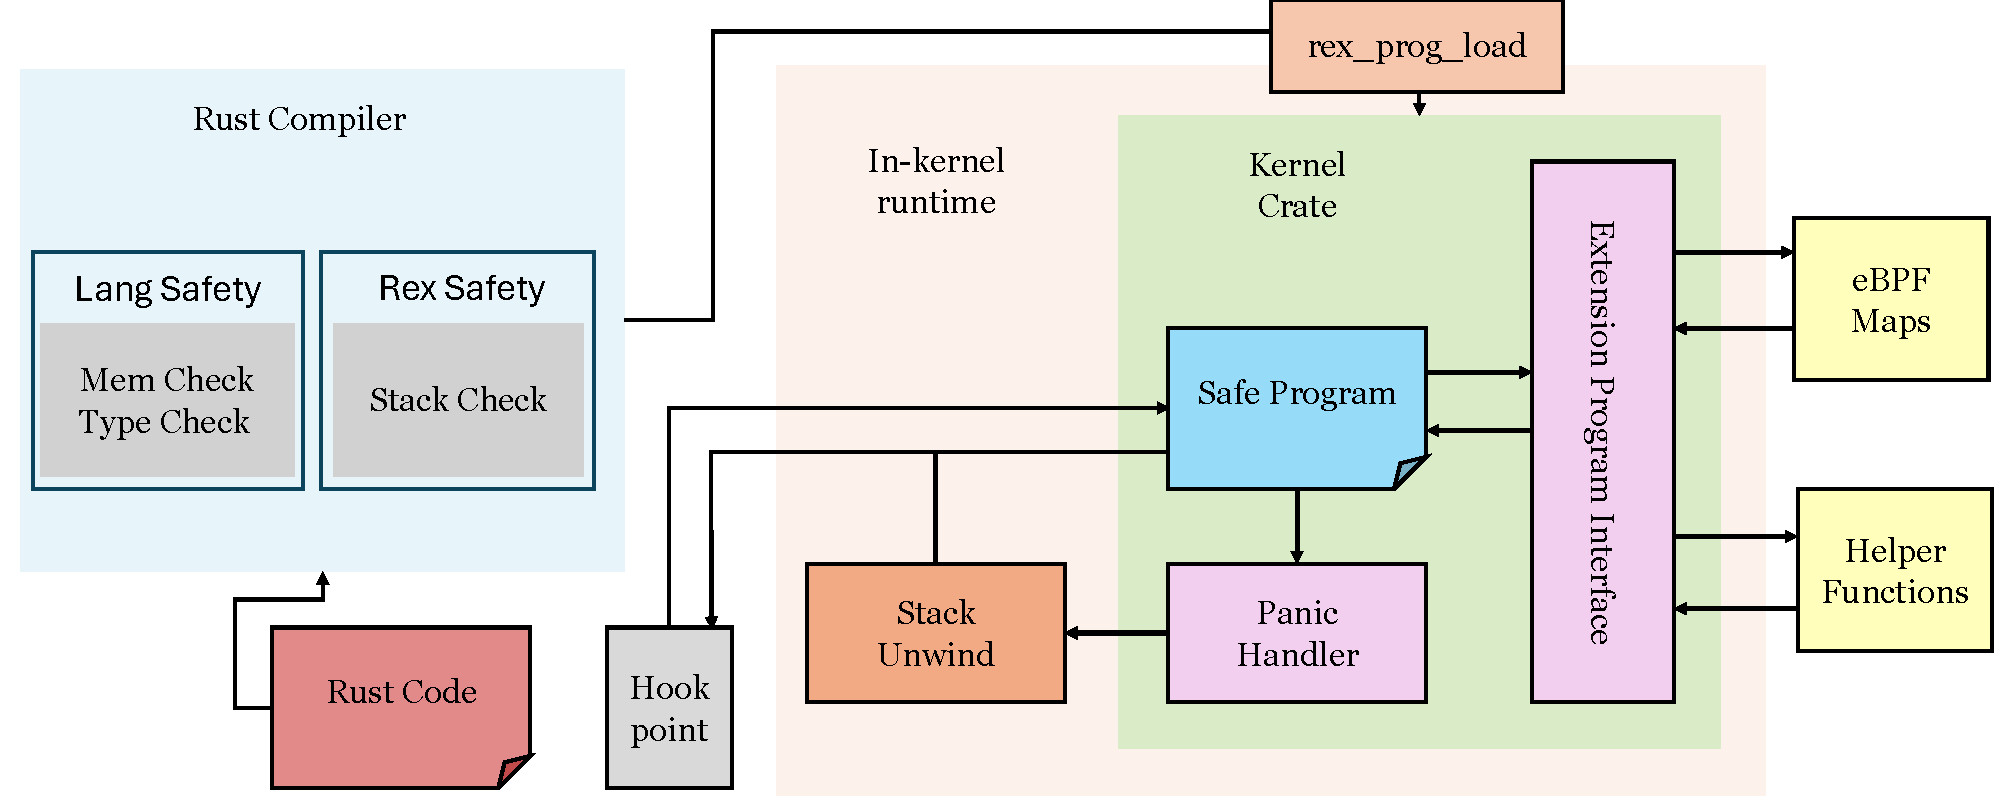
\includegraphics[width=1.0\linewidth]{figs/overview.pdf}
    \centering
    \vspace{-10pt}
    \caption{Overview of \projname{}}
    \label{fig:rex-overview}
    \vspace{-10pt}
\end{figure}

Figure~\ref{fig:rex-overview} provides an overview of the \projname{} framework.
The extension program is written strictly in safe Rust.
The program interacts with the kernel through a program interface implemented
    by the \projname{} ``kernel crate''.
The kernel crate contains unsafe Rust code due to its role as a bridge between
    the safe extension program and the unsafe but trusted kernel code.
It also provides a custom Rust panic handler to support panic-based runtime
    safety checks in Rust.
The program links with the ``kernel crate'' at compile time and runs in a
    light-weight runtime environment implemented in the kernel, which provides
    program termination and stack unwinding support.

\subsection{Ensure memory safety}
In extension programs, there are
    frequenct cases that a program needs to work on a buffer of data or a\
    specific structs.
These regions of memory are accessed by both the program and the kernel (via
    helper functions).
Rust provides powerful primitives that help to validate the memory is
    accessed correctly.
There are usually two common patterns on how the memory is accessed.
In the first case, the extension program may allocate some memory on the stack
    and send it to the kernel along with the size for processing (e.g.,
    asking kernel to fill a stack buffer with some data).
For eBPF, the verifier validates the memory region with the size to make sure
    that both the kernel and the program do not make erroneous accesses.
With Rust, its strict type safety already protects program from making a
    out-of-bound access.
In order to make sure that the size sent to the kernel is always correct, which
    is vital for the correctness of memory access from the kernel, we leverage
    the generic programming support of Rust.
For the kernel helper function that falls to the category of taking in a
    program-supplied pointer and size, the \projname{} kernel crate creates an
    adaptor interface that parametrize the type of the pointer as a generic
    type parameter.
The interface queries the size of the type from the compiler based on
    the generic type parameter and invoke the kernel interface with this size.
In this way, the size always matches the type and the kernel will make an
    out-of-bound access.
This can work for not only the scalar types, but for array types as well: Rust
    supports ``const generics'' that allows a constant to be used as a generic
    parameter, which can be used to encode array length.

In the second case, the kernel may provide the user program a piece of kernel
    memory to perform direct access (e.g., direct packet access in XDP).
The user programs must not make an out-of-bound memory access for this
    kernel-owned region of memory.
The eBPF verifier enforces user programs to explicitly check for memory
    boundaries and to not make an out-of-bound access.
In Rust, we abstract the memory region into a Rust \textit{slice} of bytes.
Rust slice provides runtime bounds checks, which allows the check to happen
    automatically without explicit handling from the program.

One challenge of supplying kernel memory to extension programs is to allow them
    to safely reinterpret the stream of bytes into useful data.
For example, a XDP program using direct packet access might need to extract
    the ethernet header information from the bytes in the packet.
Current eBPF allows the program to freely interpret the memory into other
    data types via pointer casting.
The verifier checks the casting and ensures that it does not make a pointer
    from scalar values and the new type fits in the memory chunk.
In the case of Rust, the reinterpret cast (dubbed ``transmute'' in Rust) is an
    unsafe operation, particularly because Rust does not prevent making
    pointers from scalar values.
To allow extension programs to still safely reinterpret the bytes into useful
    data types, we first define a group of primitive types that are considered
    safe as target for casting.
The safe types can be specified by implementing the \texttt{Rex::SafeTransmute}
    trait.
\projname{} requires target type of casting to be of either the safe types or a
    structure type in which all the members are of the safe types.

We use the ``proc-macro'' feature of Rust to enforce this constraint at compile
    time.
Like conventional C macros, proc-macros performs transformation on the program,
    albeit on the abstract syntax tree level.
Our proc-macro, when applied on a structure type, generates code that tries
    to treat each field of the structure as an instance of
    \texttt{Rex::SafeTransmute} followed by the actual transmute operation to
    perform the unsafe cast.
If one of field in the structure does not implement \texttt{Rex::SafeTransmute},
    the Rust compiler will issue a hard error.
At the same time, if the program tries to directly transmute the bytes into a
    structure without using the proc-macro, the compiler will also emit an
    error because tranmute belongs to unsafe Rust, which we set as forbidden
    in extension programs.
Since proc-macro transformations happen after the linting of unsafe operations,
    our proc-macro allows programs to perform transmutes in a safe, controlled
    way.

\subsection{Safely manage resources}
In addition to memory safety, extension programs must also acquire and release
    resources safely.
In eBPF, some kernel helper functions returns kernel resources that requires
    explicit release after use (e.g., reference counts of kernel objects,
    locks).
In these situations, the verifier checks the resource is released on all paths
    to prevent leaking kernel resources.

In \projname{}, the resource-acquisition-is-initialization (RAII) pattern of
    Rust can be used to create an abstraction around kernel resources that
    extension programs need.
For example, when the program obtains a spin lock from the kernel, our Rust
    abstraction layer constructs and returns a lock guard.
The lock guard implements the RAII semantics through the \texttt{drop} trait in
    Rust, which defines the operation to perform when an object is distroyed.
In the case of lock guard, its \texttt{drop} handler releases the lock.
The program does not need to explicitly release the lock or drop the loack
    guard, instead, the compile inserts an implicit \texttt{drop} at the end of
    the current scope. This effitively releases the lock when the lock guard
    goes out of scope.

\subsection{Runtime exception handling}
While the compiler contributes a lot to the safety of Rust, many safety checks
    happen at runtime in the form of exceptions (i.e., Rust panics).
In userspace, Rust uses the Itanium exception handling ABI.
When an exception is triggered, the control flow is redirected to the Rust
    panic handler in its standard library, which in turn calls into the unwind
    library to perform stack unwinding and resource cleanups for each stack
    frame.
However, the Itanium ABI is not suitable for kernel extensions, making
    exception handling a challenge in extension programs:
\begin{itemize}
    \item The Itanium ABI-based exception handling is too complicated, as the
        userspace unwind libraries are not direcly usable.
    \item Failures during unwinding, which are permissible in userspace, cannot
        be tolerated in kernel space, as incomplete cleanup means leaking
        kernel resources.
    \item ABI-based unwinding typically requires dynamic allocation, which
        creates challenges for extensions in interrupt contexts, in which an
        allocator may not be available~\cite{bpf-mempool-lwn}.
%    \item Unwinding generally executes destructors for all existing objects on
%        the stack, but executing untrusted, user-defined destructors (via the
%        \texttt{\small Drop} trait in Rust) is not safe.
\end{itemize}

\begin{figure}
	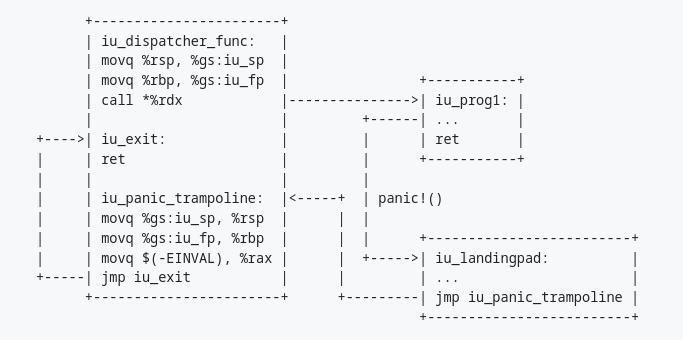
\includegraphics[width=0.8\linewidth]{figs/EH.png}
	\centering
	\vspace{-10pt}
	\caption{Overview of exception handling control flow}
	\label{fig:eh-overview}
	\vspace{-10pt}
\end{figure}

Our exception handling framework consists of two components: 1) graceful exit
    upon exceptions that resets the current context and 2) resource cleanup to
    prevent kernel resource leaks.
To support a graceful exit from an exception, we implemented a small runtime
    (as shown in Figure~\ref{fig:eh-overview}) in the kernel that contains a
    program dispatcher, a panic handler, and a landingpad function.
The dispatcher function always saves the stack and framepointer of the current
    context before calling into the program.
If the program executes normally without triggering an exception, it would just
    return normally and then return from the dispatcher.
Under exceptional cases where a Rust panic is triggered, the panic handler will
    transfer the control flow to the landingpad function to print debug
    information related to the exception (e.g., exception message) to the
    kernel ring buffer.
Then, the landingpad function redirects the control flow to a pre-defined label
    in the dispatcher function, where it restores the old value of the stack
    and frame pointer from the storage location.
This effectively unwinds the stack and resets the context as if the extension
    program returned successfully.

For resource cleanup, light-weight mechanisms can be effective.
Our insight for resource cleanup is that the extension program can only obtain
    resources by explicitly issuing helper function calls and therefore only
    these resources needs to be released.
For these helper function calls, we record the allocated kernel resource during
    execution.
Upon a panic, the panic handler will take the responsiblility to correctly
    handle the release of kernel resources.
We implement the cleanup code as part of our extension programming interface
    and programs themselves do not need to handle cleanups.

\subsection{Safe guard the kernel stack}
One unique safety requirement the kernel extension programs are facing is the
    usage of kernel stack.
Unlike the userspace programs, where the stack can grow indefinitely on demand (\jinghao{TODO: add a footnote}),
    the stack in kernel space is fix-sized (4 pages on X86-64) and therefore
    limited.
Overflowing the kernel stack may result in memory corruptions or kernel panics.

The stack safety property is checked in eBPF.
The eBPF verifier handles it by keeping track of the stack size throughout its
    symbolic execution process.
However, the verification of the stack usage does not always yield the correct
    result -- in particular, the verifier fails to track stack usage across the
    indirect tail calls.

Our observation is that the enforcement of stack safety is easier to check at
    runtime when indirect or recursive calls are present in the code.
\projname{} takes a hybrid approach in ensuring stack safety that employs
    static checks for programs without indirect or recursive calls, and
    dynamic, runtime checks for programs make use of these function calls.
For each program being compiled, the \projname{}-specific pass in the compiler
    will check whether it involves indirect or recursive calls.
When the extension program contains only direct, non-recursive function calls,
    its total stack usage can be calculated by traversing its static callgraph.
If the total stack usage of the program exceeds total amount of stack
    available, the \projname{} compiler pass will generate an error and reject
    the program.

On the other hand, programs with indirect or recursive calls are hard to be
    checked for stack usage statically, as is the case in the eBPF verifier.
In these cases, \projname{} performs runtime checks to limit the stack usage of
    programs.
The \projname{} compiler pass first ensures each function in the program takes
    less than one page of stack.
Then, before each function call in the extension program, the \projname{}
    compiler pass inserts a call to \texttt{\_\_rex\_check\_stack} function.
\texttt{\_\_rex\_check\_stack} is provided by the kernel crate and checks the
    current stack depth of the program, if the stack usage exceeds the
    threshold, it will trigger a Rust panic and effectively terminate the
    program.

\projname{} defines the stack usage threshold to be two pages less than the
    total stack available.
This design choice is based on two considerations.
First, kernel helper functions are not visible at program compile time but they
    also account for stack usage during program execution.
Leaving extra spaces accomdates kernel helper functions and we believe two
    pages of stack is a reasonable limit for kernel helper functions.
Second, since the stack usage of each function in the program is limited to
    1 page of stack, in the worse case the remaining stack space is at least
    one page when \texttt{\_\_rex\_check\_stack} triggers a Rust panic.
This worse case guarrantee leaves enough space for the panic handling and stack
    unwinding routines.